%
% teil5.tex -- Beispiel-File für Teil 5
%
% (c) 2020 Prof Dr Andreas Müller, Hochschule Rapperswil
%
% !TEX root = ../../buch.tex
% !TEX encoding = UTF-8
%
\section{Rücktransformation (ICWT)
	\label{wavelets:section:teil5}}
\rhead{Teil 5}

In diesem kurzen Abschnitt wird die Rücktransformation vom Frequenz- in den Zeitbereich betrachtet. Dabei wird die erhaltene $a_n$ x $b_m$ Matrix (aus der CWT), welche die Transformationsparameter im Bildbereich beinhaltet in den Zeitbereich rücktransformiert. Dabei sollte in dieser Betrachtung wieder das Ausgangssignal aus der Abbildung \ref{wavelet:fig:FFTnoiseFree} zurück gewonnen werden.
Das erhaltene Resultat aus der ICWT Abbildung \ref{wavelet:fig:ICWT}, entpricht aber nicht wirklich dem eingangs transformierten Signal, weil:

\begin{itemize}
	\item die CWT ein verschmiertes Spektrum erzeugt.
	\item das Morlet Wavelet einem Gauss gewichteten Cosinus entspricht und damit kein scharfkantiges Sinus- oder Cosinussignal reproduziert werden kann.
\end{itemize}

Um letztere These genauer zu untersuchen, wurden zwei Wege eingeschlagen. Zum einen die Rücktransformation des Cosinus über dasselbe Gauss Fenster mit dem schon das Wavelet generiert wurde und zum anderen mit einem Rechteckfenster, in der Hoffnung das dieses einen reines Sinus Signal besser reproduzieren kann.

Abbildung \ref{wavelet:fig:ICWT} zeigt aber, dass die Problematik in erster Linie beim verschmieren der Frequenzausgabe liegt. Die CWT detektiert die Frequenz nicht gleich scharf wie die FFT und dadurch werden Frequenzen nahe der Hauptfrequenz ebenfalls mit einer nennenswerten Amplitude im Frequenzspektrum angegeben. Bei Rücktransformation werden diese Anteile mit einbezogen und verursachen eine Überlagerung (analog zur Abbildung \ref{wavelet:fig:AmplitudengangExtraktionDFT} unten). Diese Interferenz verhindert Hauptsächlich die Möglichkeit mit der CWT eine sinnvolle Rücktransformation zu erhalten. Aus Zeit gründen konnten hier auch keine weiteren Versuche für eine Optimierung gestartet werden. In gemachten ICWT wurde die Mittlung noch vernachlässigt, wodurch die Amplitudenwerte durch die Aufsummierung der einzelnen spektralen Anteile stark überhöht sind.

\begin{figure}
	\centering
	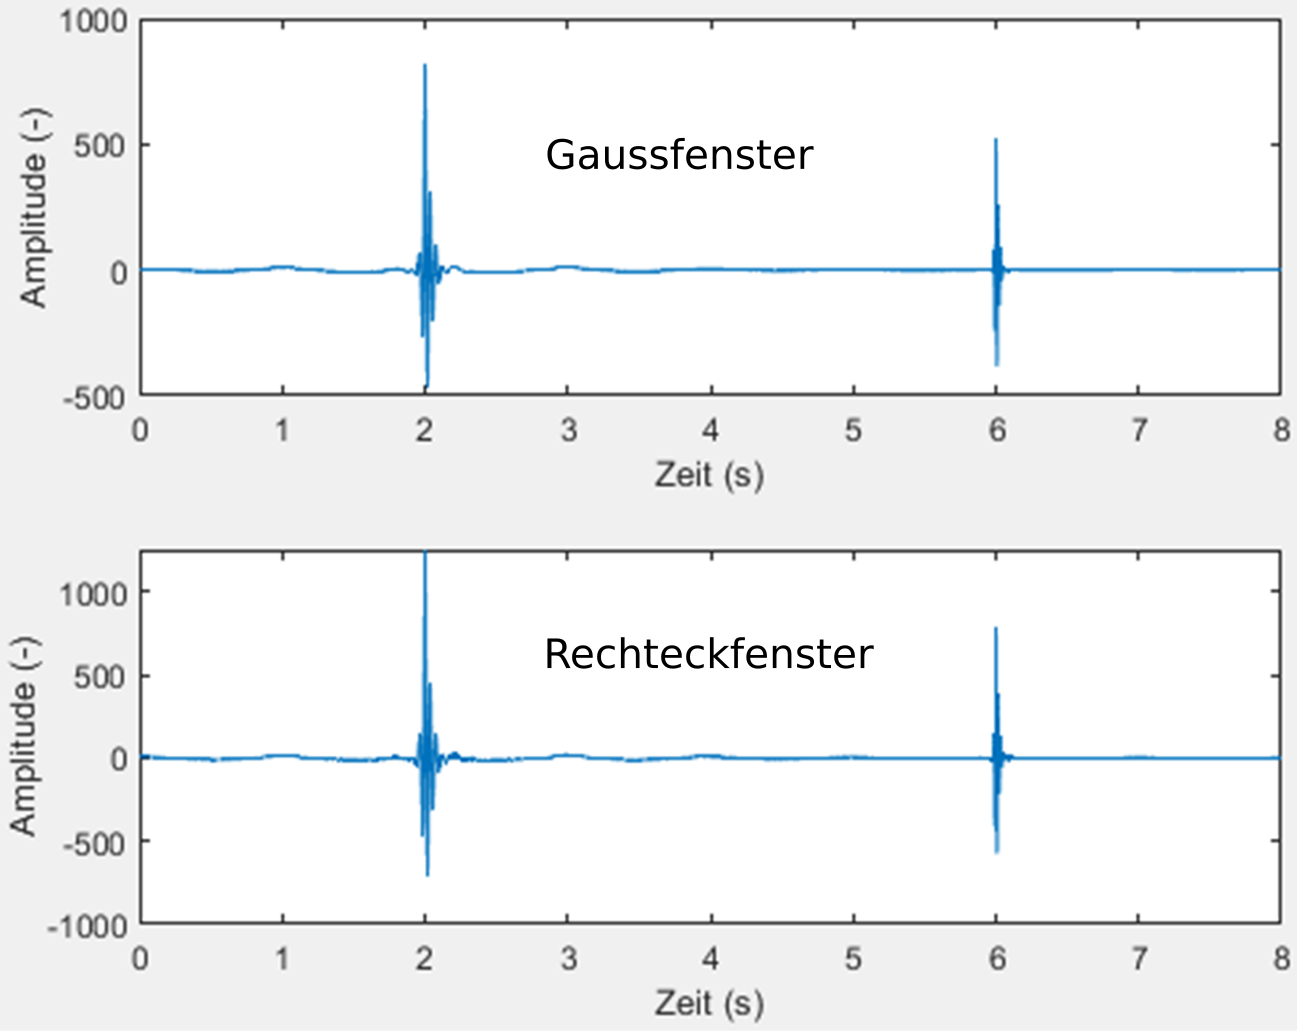
\includegraphics[width=0.5\textwidth]{papers/wavelets/images/19-1_ICWT.png}
	\caption{Rücktransformation des CWT transformierten Testsignal aus Abbildung \ref{wavelet:fig:FFTnoiseFree}. Einerseits mittels des Wavelets selbst und andererseits mit der Verrechnung der CWT-Matirx mit einem Rechteckfenster (anstatt des Gauss Fensters).}
	\label{wavelet:fig:ICWT}
\end{figure}